\documentclass[a4paper]{scrartcl}
% Use small margins
\usepackage[left=1.5cm, right=1.5cm, top=1cm, bottom=2cm]{geometry}
\usepackage[unicode,
            pdfencoding=auto,
            pdfinfo={
              Title={Sprawozdanie z Generatorów},
              Author={Maciej Mionskowski},
              Subject={Sprawozdanie Generator},
              Keywords={},
              Producer={xelatex},
            },
]{hyperref}
\usepackage[T1]{fontenc}
\usepackage{polski}
\usepackage[polish]{babel}
\usepackage[utf8]{inputenc}
\usepackage{upgreek}
\usepackage{array}
\usepackage{amsmath}
\usepackage{mathtools}
\usepackage{caption}
\usepackage{subcaption}
\usepackage{tabularx}
\usepackage{graphicx}
\usepackage{subfig}
\graphicspath{ {images/} }
\renewcommand{\arraystretch}{1.5}
\setlength{\abovedisplayskip}{5pt}

\author{Maciej Mionskowski}
\title{Sprawozdanie 4}
\date{}
\subtitle{Generator}
\begin{document}
	{\let\newpage\relax\maketitle}
	{\begin{center}Celem ćwiczenia było zapoznanie się, poprzez badania symulacyjne, z działaniem generatorów relaksacyjnych wykorzystujących wzmacniacz operacyjny z pętlą dodatniego sprzężenia zwrotnego.\end{center}}
	\begin{section}{Generator relaksacyjny ze wzmacniaczem operacyjnym}
		\begin{subsection}{Cel}
			Celem ćwiczenia było zbadanie wpływu zmiany wartości komponentów w układzie takich jak: rezystor, kondensator; na napięcie wyjściowe i częstotliwość drgań rezystora w układzie generatora relaksacyjnego ze wzmacniaczem operacyjnym.
		\end{subsection}
		\begin{subsection}{Analiza}
				\begin{figure}[ht]
				\begin{center}
					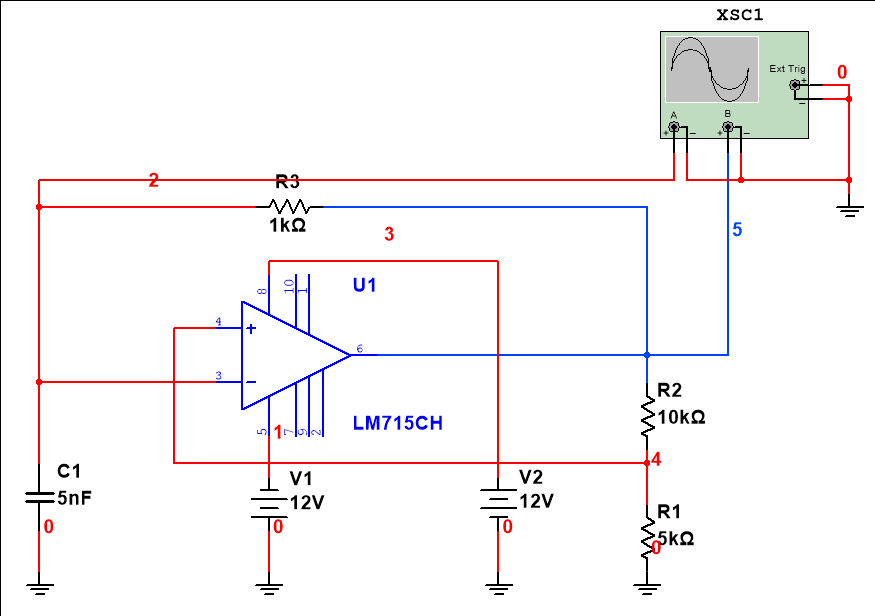
\includegraphics[width=0.8\linewidth]{03-circuit}
					\caption{Schemat ideowy generatora relaksacyjnego ze wzmacniaczem operacyjnym.}
					\label{fig:circuit-1}
				\end{center}
				\end{figure}

				\begin{figure}[!ht]
				\begin{center}
					\begin{subfigure}{.45\textwidth}
						\begin{center}
						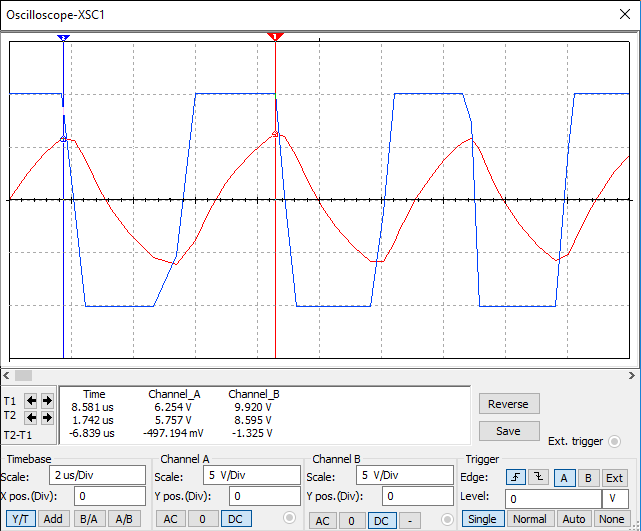
\includegraphics[width=\linewidth,scale=2]{03-period}
						\caption{Pomiar okresu $ \frac{1}{T} = f $ w obwodzie \ref{fig:circuit-1} przy wartościach komponentów jak na rysunku.}
						\label{fig:exercise-2-punkt-pracy}
						\end{center}
					\end{subfigure}
					\begin{subfigure}{.45\textwidth}
						\begin{center}
						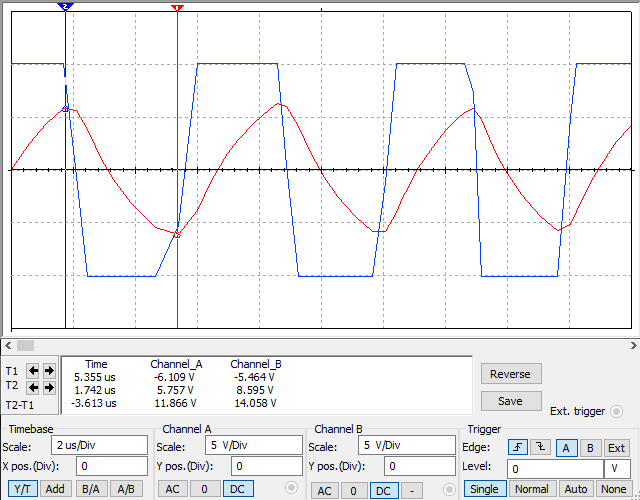
\includegraphics[width=\linewidth,scale=2]{03-ucminmax}
						\caption{Pomiar napięcia na kondensatorze $u_{c} $ w obwodzie \ref{fig:circuit-1} przy wartościach komponentów jak na rysunku.}
						\label{fig:exercise-2-punkt-pracy}
						\end{center}
					\end{subfigure}
				\end{center}
				\caption{Pomiary napięć i okresu (częstotliwości) w obwodzie. Wyniki obserwacji z powyższych zrzutów znajdują się w wierszu 1. tabelki poniżej.}
				\end{figure}

				\begin{table}[!ht]
					\begin{center}
					\caption{Wartości zmierzone w obwodzie na rysunku \ref{fig:circuit-1} przy zmianie wartości rezystora $ R_{1} $}
					\begin{tabular}{| l | l | l | l | l | r |}
						\hline
						$ R_{1} $ & $ R_{2} $ & $ u_{c_{min}} $ & $ u_{c_{max}} $ & $ \Delta T $ & $ f $ \\ \hline
						$ 5\mathrm{k\Omega} $ & $ 10\mathrm{k\Omega} $ & $ -6.079\mathrm{V} $ & $ 6.254\mathrm{V} $ & $ 6.839 \mathrm{\mu s} $ & $ 146.22 \mathrm{kHz} $ \\ \hline
						$ 10\mathrm{k\Omega} $ & $ 10\mathrm{k\Omega} $ & $ -7.4\mathrm{V} $ & $ 7.312\mathrm{V} $ & $ 8.324 \mathrm{\mu s} $ & $ 120.13 \mathrm{kHz} $ \\ \hline
						$ 20\mathrm{k\Omega} $ & $ 10\mathrm{k\Omega} $ & $ -8.8\mathrm{V} $ & $ 8.304\mathrm{V} $ & $ 11.2 \mathrm{\mu s} $ & $ 89.285 \mathrm{kHz} $ \\ \hline
						$ 40\mathrm{k\Omega} $ & $ 10\mathrm{k\Omega} $ & $ -10\mathrm{V} $ & $ 8.8\mathrm{V} $ & $ 12.82 \mathrm{\mu s} $ & $ 78\mathrm{kHz} $ \\ \hline
					\end{tabular}
					\end{center}
				\end{table}
				
				\begin{table}[!htbp]
					\begin{minipage}{0.465\linewidth}
					\centering
					\caption{Wartości zmierzone w obwodzie na rysunku \ref{fig:circuit-1} przy zmianie wartości rezystora $ R_{3} $}
					\hfill
					\begin{tabular}{| l | l | l | r |}
						\hline
						$ R_{3} $ & $ C $ & $ \Delta T $ & $ f $ \\ \hline
						$ 1\mathrm{k\Omega} $ & $ 2\mathrm{nF} $ & $ 8.387 \mathrm{\mu s} $ & $ 119.232 \mathrm{kHz} $ \\ \hline
						$ 5\mathrm{k\Omega} $ & $ 2\mathrm{nF} $ & $ 22.742 \mathrm{\mu s} $ & $ 43.971 \mathrm{kHz} $ \\ \hline
						$ 10\mathrm{k\Omega} $ & $ 2\mathrm{nF} $ & $ 36.53 \mathrm{\mu s} $ & $ 27.374 \mathrm{kHz} $ \\ \hline
						$ 20\mathrm{k\Omega} $ & $ 2\mathrm{nF} $ & $ 67 \mathrm{\mu s} $ & $ 14.925 \mathrm{kHz} $ \\ \hline
					\end{tabular}
					\end{minipage}\hfill
					\begin{minipage}{0.45\linewidth}
					\centering
					\caption{Wartości zmierzone w obwodzie na rysunku \ref{fig:circuit-1} przy zmianie wartości kondensatora $ C $}
					\hfill
					\begin{tabular}{| p{1.6cm} | l | r |}
						\hline
						$ C $ & $ \Delta T $ & $ f $ \\ \hline
						$ 2\mathrm{nF} $ & $ 8.387 \mathrm{\mu s} $ & $ 119.232 \mathrm{kHz} $ \\ \hline
						$ 5\mathrm{nF} $ & $ 13.548 \mathrm{\mu s} $ & $ 73.811 \mathrm{kHz} $ \\ \hline
						$ 10\mathrm{nF} $ & $ 22.581 \mathrm{\mu s} $ & $ 44.285 \mathrm{kHz} $ \\ \hline
						$ 20\mathrm{nF} $ & $ 39.032 \mathrm{\mu s} $ & $ 25.620 \mathrm{kHz} $ \\ \hline
					\end{tabular}
					\end{minipage}
				\end{table}
				\pagebreak
		\end{subsection}
		\begin{subsection}{Wniosek}
			Generator relaksacyjny oparty na wzmacniaczu operacyjnym generuje niezbyt dokładny sygnał wyjściowy prostokątny. Na częstotliwość sygnału wyjściowego wpływa wiele komponentów układu. Podczas analizy zajęliśmy się rezystorami $ R_{1}, R_{2} $ i kondensatorem $ C $. Wraz ze wzrostem rezystancji któregokolwiek z rezystorów częstotliwość maleje, a amplituda napięcia $ u_{c} $ rośnie. Analogicznie wzrost pojemności kondensatora $ C $ powoduje zmniejszenie częstotliwości drgań.
		\end{subsection}
	\end{section}
	\newpage

	\begin{section}{Generator relaksacyjny z dwoma progami komparacji.}
		\begin{subsection}{Cel}
			Celem ćwiczenia było zapoznanie z budową i zasadą działania generatora relaksacyjnego z dwoma progami komparacji, a także sprawdzenie wpływu zmian wartości komponentów na wyjście generatora.
		\end{subsection}

		\begin{subsection}{Analiza}
				\begin{figure}[!ht]
				\begin{center}
					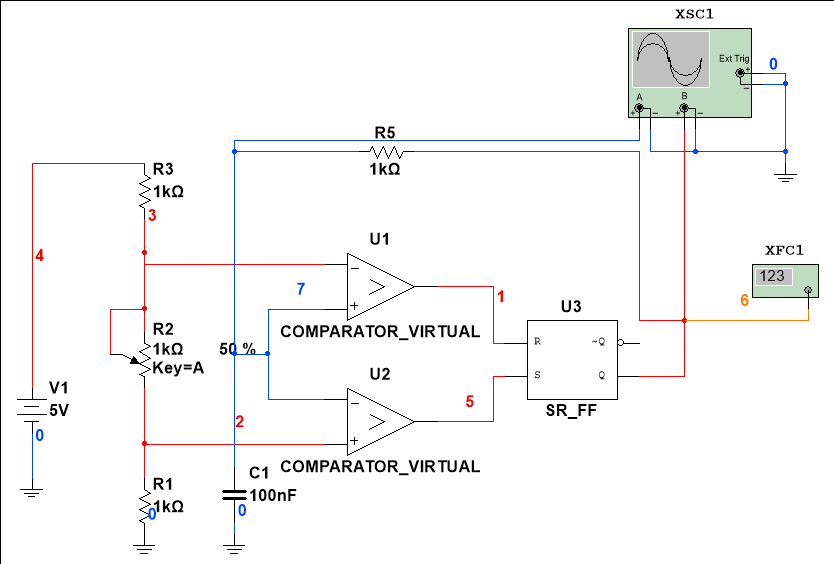
\includegraphics[width=0.7\linewidth,scale=2]{04-circuit}
					\caption{Układ generatora relaksacyjnego z dwoma progami komparacji.}
					\label{fig:04-circuit}
				\end{center}
				\end{figure}

				\begin{figure}[!ht]
				\begin{center}
					\begin{subfigure}{.63\textwidth}
						\begin{center}
						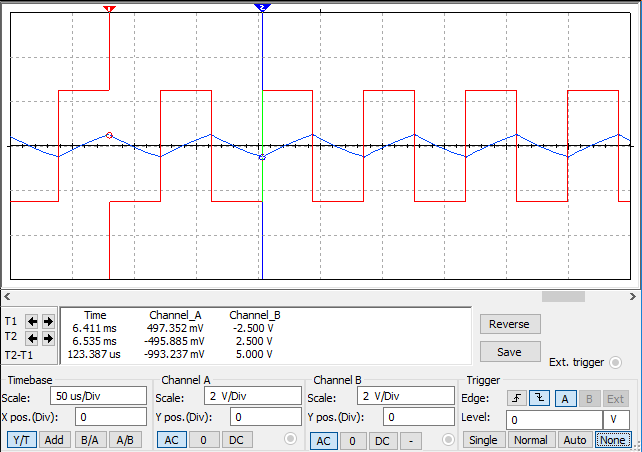
\includegraphics[width=\linewidth,scale=2]{04-osciloscope}
						\caption{Przebieg na kondensatorze $ C $ i wyjściu w układzie na rysunku \ref{fig:04-circuit}. Widać jak zmienia się stan wraz ze zmianą napięcia na kondensatorze.}
						\end{center}
					\end{subfigure}%
					\begin{subfigure}{.35\textwidth}
						\begin{center}
						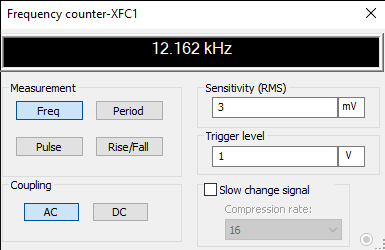
\includegraphics[width=\linewidth,scale=2]{04-freq}
						\caption{Pomiar częstotliwości sygnału wyjściowego obwodzie \ref{fig:04-circuit} przy wartościach komponentów jak na rysunku.}
						\end{center}
					\end{subfigure}
				\end{center}
				\caption{Pomiary napięć i częstotliwości w obwodzie dla $ R_{2} = 50\%*1\mathrm{k\Omega} $. Wyniki obserwacji z powyższych zrzutów znajdują się w wierszu 2. tabelki poniżej.}
				\end{figure}

				\begin{table}[!ht]
					\begin{center}
					\caption{Wartości zmierzone w obwodzie na rysunku \ref{fig:04-circuit} przy zmianie wartości rezystora $ R_{2} $. Wraz ze spadkiem rezystancji rośnie częstotliwość.}
					\begin{tabular}{| l | l | l | l | r |}
						\hline
						$ R_{2} $ & $ U_{p1} $ & $ U_{p2} $ & $ U_{p1} - U_{p2} $ & $ f $ \\ \hline
						$ 100\mathrm{\%} * 1\mathrm{k\Omega} $ & $ 3.333\mathrm{V} $ & $ 1.667\mathrm{V} $ & $ 1.666\mathrm{V} $ & $ 7.157 \mathrm{kHz} $ \\ \hline
						$ 50\mathrm{\%} * 1\mathrm{k\Omega} $ & $ 3\mathrm{V} $ & $ 2\mathrm{V} $ & $ 1\mathrm{V} $ & $ 12.162 \mathrm{kHz} $ \\ \hline
						$ 25\mathrm{\%} * 1\mathrm{k\Omega} $ & $ 2.778\mathrm{V} $ & $ 2.222\mathrm{V} $ & $ 0.556\mathrm{V} $ & $ 21.7514 \mathrm{kHz} $ \\ \hline
						$ 0\mathrm{\%} * 1\mathrm{k\Omega} $ & $ 2.5\mathrm{V} $ & $ 2.5\mathrm{V} $ & $ 0\mathrm{V} $ & $ 71.7514 \mathrm{kHz} $ \\ \hline
					\end{tabular}
					\end{center}
				\end{table}

				\begin{figure}[!ht]
					\begin{center}
						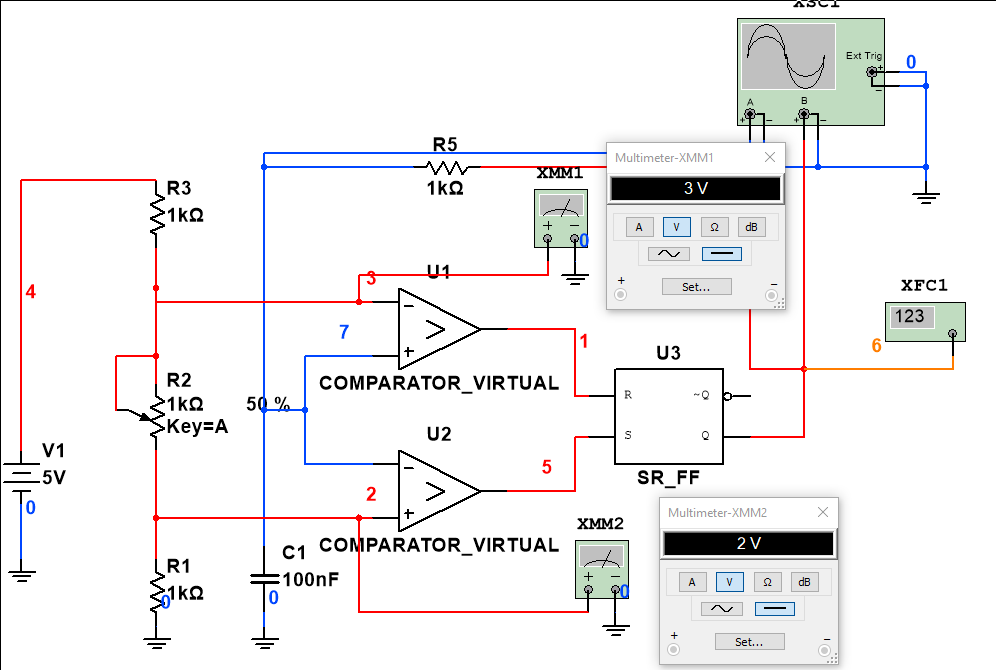
\includegraphics[width=.75\linewidth]{04-base-progi}
						\caption{Progi komparacji dla $ R_{2} = 50\%*1\mathrm{k\Omega}$ }
					\end{center}
				\end{figure}

				\begin{figure}[!ht]
					\begin{center}
						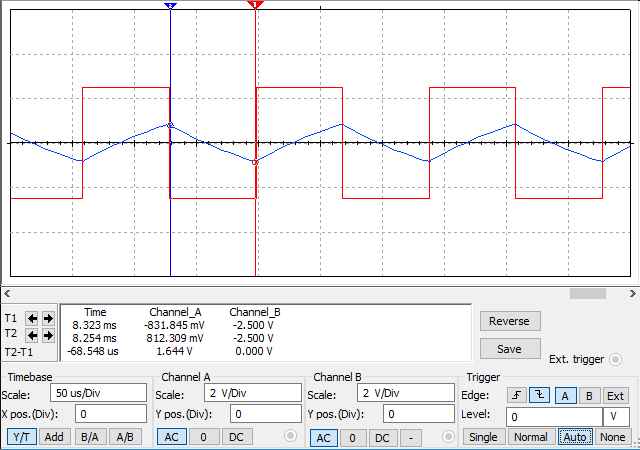
\includegraphics[width=.6\linewidth]{04-100proc-osc}
						\caption{Przebieg napięcia na kondensatorze i sygnału wyjścia dla $ R_{2} = 100\%*1\mathrm{k\Omega}$ }
					\end{center}
				\end{figure}

				\begin{figure}[!ht]
					\begin{center}
						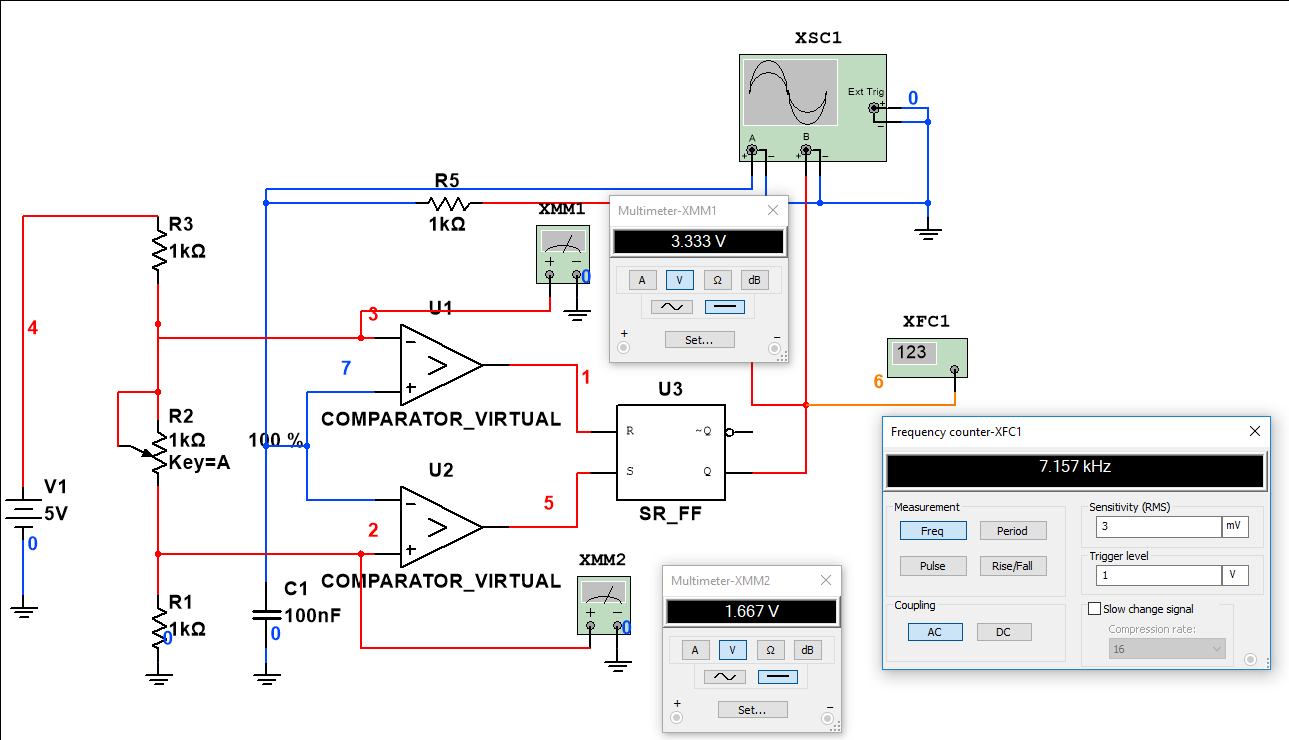
\includegraphics[width=.8\linewidth]{04-100proc1k-progi}
						\caption{Progi komparacji dla $ R_{2} = 100\%*1\mathrm{k\Omega}$ }
					\end{center}
				\end{figure}
				\pagebreak
		\end{subsection}
		\begin{subsection}{Wniosek}
			Generator progowy z dwoma progami komparacji działa dzięki kondensatorowi umieszczonemu w układzie. Okresowo prąd zmienia kierunek, którym płynie. Raz kondensator się rozładowuje, a raz ładuje. Zastosowanie dwóch progów komparacji pozwala dość dokładnie kontrolować częstotliwość. W układzie z ćwiczenia użyliśmy dzielnika napięcia aby regulować progi komparacji. Wraz ze spadkiem rezystancji wzrasta częstotliwość (częściej przełączają się komparatory). Wpływ na częstotliwość podobnie jak w zadaniu pierwszym ma pojemność kondensatora i wartość na potencjometrze między progami komparacji.
		\end{subsection}
	\end{section}

	\begin{section}{Generator sterowany napięciem VCO (Voltage Controlled Oscillator)}
		\begin{subsection}{Cel}
			Celem ćwiczenia było zbudowanie na bazie generatora z dwoma programi komparacji generatora sterowanego napięciem i zaobserwowaniem reakcji obwodu na zmiany parametrów.
		\end{subsection}
		\begin{subsection}{Analiza}
				\begin{figure}[ht]
				\begin{subfigure}{0.75\linewidth}
				\begin{center}
					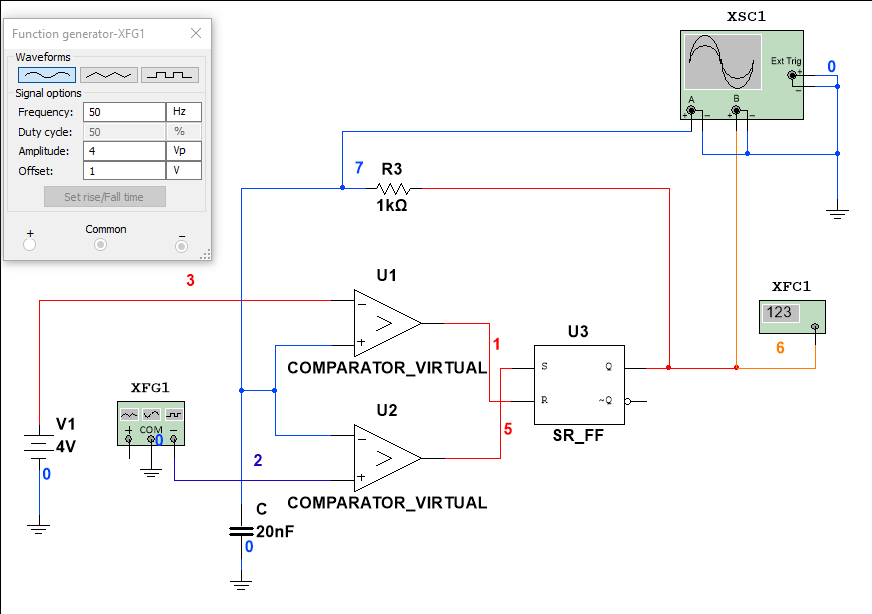
\includegraphics[width=0.74\linewidth]{05-circuit}
				\end{center}
				\end{subfigure}%
				\begin{subfigure}{0.25\linewidth}
				\begin{center}
					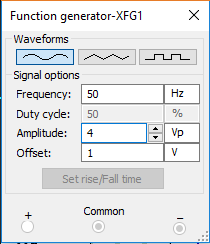
\includegraphics[width=\linewidth]{05-func}
				\end{center}
				\end{subfigure}
				\caption{Schemat ideowy generatora sterowanego napięciem - VCO.}
				\label{fig:circuit-05}
				\end{figure}

				\begin{figure}[!ht]
				\begin{center}
					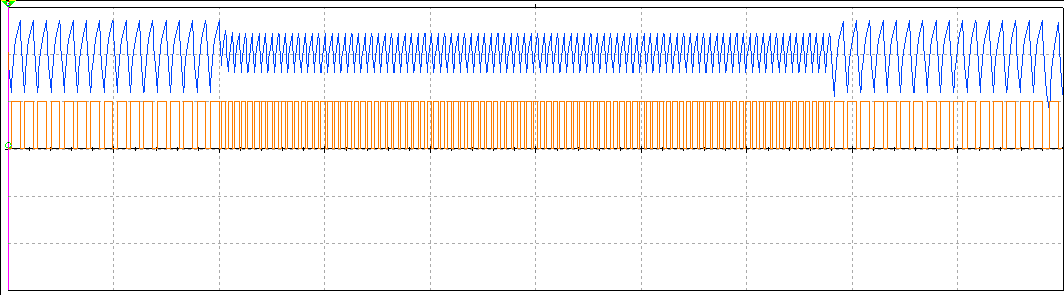
\includegraphics[width=\linewidth]{05-out}
					\caption{Pomiar napięcia na kondensatorze (niebieski) i wyjście (pomarańczowy). Pomiar na kondensatorze został przesunięty na osi w górę, aby wykres był czytelny. Widać, że czym szybsza oscylacja na oscyloskopie tym gęstszy sygnał dostajemy na wyjściu. $ A=4\rmmath{V} $}
				\end{center}
				\end{figure}

				\begin{figure}[!ht]
				\begin{center}
					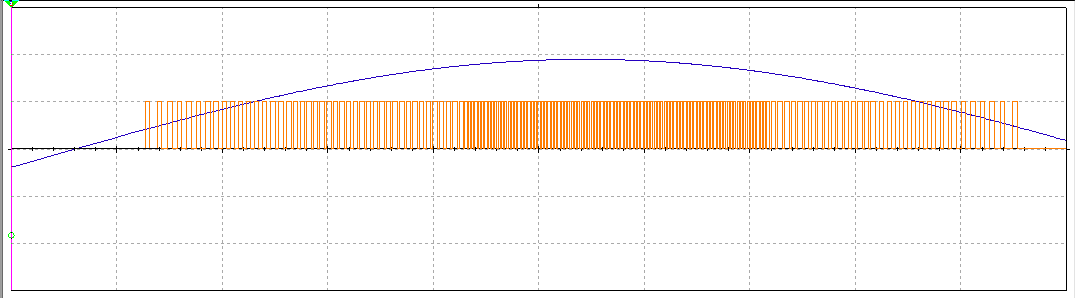
\includegraphics[width=\linewidth]{05-gen-out}
					\caption{Pomiar napięcia na generatorze (niebieski) i wyjście (pomarańczowy). Pomiar na generatorze został przesunięty na osi w górę, aby wykres był czytelny. Widać, że czym większe napięcie na wejściu generatora, a więc wejściu komparatora tym sygnał na wyjściu jest gęściej upakowany. Pomiar dla wartości jak na obwodzie na rysunku \ref{fig:circuit-05}}
				\end{center}
				\end{figure}

				\begin{figure}[!ht]
				\begin{center}
					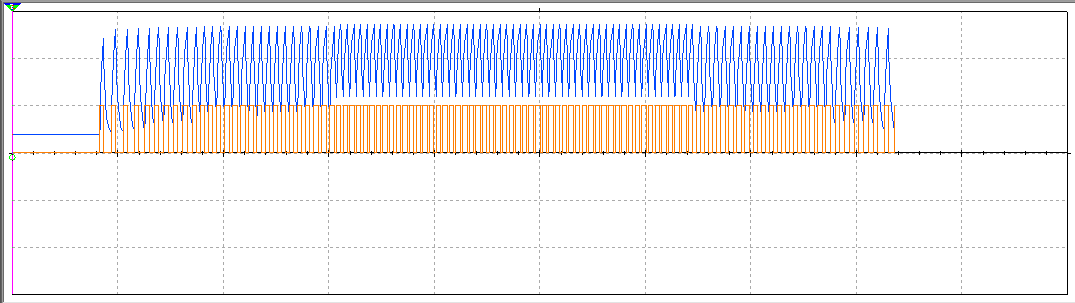
\includegraphics[width=\linewidth]{05-osc-3v}
					\caption{Pomiar napięcia na kondensatorze (niebieski) i wyjście (pomarańczowy). Pomiar na kondensatorze został przesunięty na osi w górę, aby wykres był czytelny. Zmniejszenie amplitudy poskutkowało zmniejszeniem częstotliwości sygnału wyjściowego. $ A=3\rmmath{V} $}
				\end{center}
				\end{figure}
		\end{subsection}
		\begin{subsection}{Wniosek}
			Na przebiegach obserwowanych na oscyloskopie jasno wynika jak generator sterowany napięciem (VCO) reaguje na zmianę napięcia na generatorze. Czym wyższe napięcie na generatorze tym gęściej upakowany sygnał. Taki układ może służyć na przykład do modulacji FM.
		\end{subsection}
	\end{section}
\end{document}
